\documentclass{standalone}
\usepackage{pgfplots}
\begin{document}
\pgfplotsset{ticks=none}
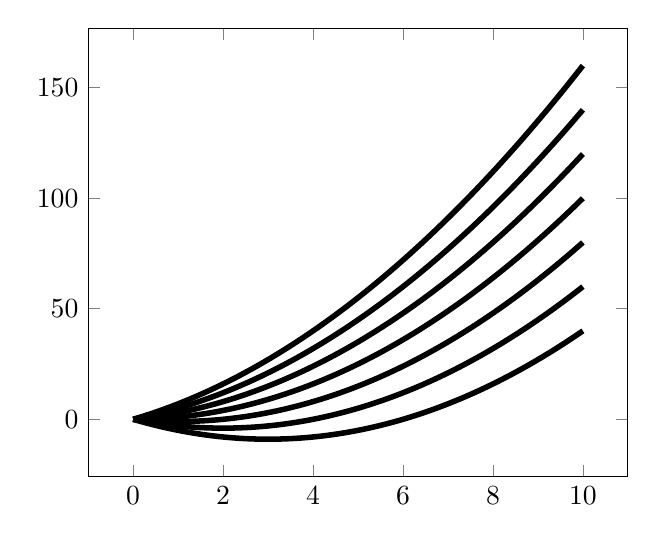
\begin{tikzpicture}
  \begin{axis}%[hide axis]
    \addplot[smooth, samples=100, line width = 2, domain=0:10] 
    (\x,{\x^2 + 6*\x});
    \addplot[smooth, samples=100, line width = 2, domain=0:10] 
    (\x,{\x^2 + 4*\x});
    \addplot[smooth, samples=100, line width = 2, domain=0:10] 
    (\x,{\x^2 + 2*\x});
    \addplot[smooth, samples=100, line width = 2, domain=0:10] 
    (\x,{\x^2 - 0*\x});
    \addplot[smooth, samples=100, line width = 2, domain=0:10] 
    (\x,{\x^2 - 2*\x});
    \addplot[smooth, samples=100, line width = 2, domain=0:10] 
    (\x,{\x^2 - 4*\x});
    \addplot[smooth, samples=100, line width = 2, domain=0:10] 
    (\x,{\x^2 - 6*\x});
  \end{axis}
\end{tikzpicture}
\end{document}